%%\documentclass[finalspec]{sbmlpkgspec}
\documentclass[draftspec]{sbmlpkgspec}
\usepackage{microtype}
\usepackage{color}

\usepackage{todonotes}
\usepackage{subfigure}
\usepackage{longtable}

\usepackage[final]{pdfpages}

%% ============================================================================
%% Description:  Documentation for sbmlpkgspec.cls
%% First author: Michael Hucka <mhucka@caltech.edu>
%% Organization: California Institute of Technology
%% Date created: September 2011
%% https://sbml.svn.sourceforge.net/svnroot/sbml/trunk/project/tex/sbmlpkgspec
%%
%% Copyright (C) 2011-2012 California Institute of Technology, Pasadena, CA.
%%
%% SBMLPkgSpec is free software; you can redistribute it and/or modify it
%% under the terms of the GNU Lesser General Public License as published by
%% the Free Software Foundation.  A copy of the license agreement is provided
%% in the file named "LICENSE.txt" included with this software distribution.
%% ============================================================================

% Macros just for this document:

\newcommand{\rfcnum}{{115}}

\newcommand{\sbmlpkg}{\texorpdfstring{%
    \textls[-25]{\textsc{SBMLPkgSpec}}}{%
    \textsc{SBMLPkgSpec}}\xspace}
\newcommand{\sbmlpkghead}{\texorpdfstring{%
    \textls[-50]{\textsc{SBMLPkgSpec}}}{%
    \textsc{SBMLPkgSpec}}\xspace}
\newcommand{\sbmlpkgfile}{\literalFont{sbmlpkgspec.cls}\xspace}
\newcommand{\latex}{\LaTeX{}\xspace}
\newcommand{\tex}{\TeX{}\xspace}
\newcommand{\distURL}{http://sourceforge.net/projects/sbml/files/specifications/tex}
\newcommand{\srcURL}{https://sbml.svn.sourceforge.net/svnroot/sbml/trunk/project/tex/sbmlpkgspec}
\newcommand{\webURL}{http://sbml.org/Documents/Specifications/The_SBMLPkgSpec_LaTeX_class}
\newcommand{\cmd}[1]{\literalFont{\textbackslash #1}}

% Custom latex listing style, for use with the listings package.  The default
% highlights far too many things, IMHO.  This keeps it simple and only adjusts
% the appearance of comments within listings.

\lstdefinelanguage{mylatex}{%
  morekeywords={},%
  sensitive,%
  alsoother={0123456789$_},%$
  morecomment=[l]\%%
}[keywords,tex,comments]

\lstdefinestyle{latex}{language=mylatex}


%Listing style for SBOL RDF/XML serialization examples
\usepackage{listings}
\usepackage{color}
\usepackage{xcolor} 
\definecolor{dkgreen}{rgb}{0,0.6,0}
\definecolor{gray}{rgb}{0.5,0.5,0.5}
\definecolor{light-gray}{gray}{0.97}
\lstdefinelanguage{sbol}
    {morekeywords={xmlns:sbol,rdf:about,sbol:displayId,sbol:persistentIdentity,sbol:version,sbol:timeStamp,sbol:name,sbol:description,sbol:member,sbol:Collection,sbol:type, sbol:role, sbol:ComponentDefinition, sbol:MapsTo, sbol:sequence,sbol:wasDerivedFrom,sbol:Component,sbol:subComponent,sbol:SequenceAnnotation,sbol:component,sbol:location, sbol:sequenceAnnotation, sbol:Range, sbol:start, sbol:end, sbol:orientation,sbol:SequenceConstraint, sbol:restriction, sbol:subject, sbol:object,sbol:Sequence, sbol:elements, sbol:encoding,sbol:Model, sbol:source, sbol:language, sbol:framework,sbol:FunctionalComponent, sbol:Module, sbol:Interaction, sbol:interaction, sbol:module, sbol:model,sbol:Model,sbol:definition, sbol:access, sbol:direction, sbol:mapsTo, sbol:refinement, sbol:local, sbol:remote, sbol:participation, sbol:Participation, sbol:participant,sbol:sequenceConstraint,sbol:at,sbol:Cut,sbol:functionalComponent,sbol:ModuleDefinition,prov:wasDerivedFrom,dcterms:title,dcterms:description},
     basicstyle=\fontsize{7}{9}\selectfont\ttfamily,
     backgroundcolor=\color{light-gray},
     keywordstyle=\color{blue},
     commentstyle=\color{gray},
     stringstyle=\color{dkgreen},
     tabsize=2,
     showspaces=false,
     showstringspaces=false,
     breaklines=true,                           % wrap text
     sensitive=true,                            % keywords are case sensitive
     %morecomment=[l][commentstyle]{\#},         % comment format
     morestring=[b]",                           % string format
     escapeinside={[}{]},
     alsoletter=:
     %breakatwhitespace=true, 
     %literate={\-}{}{0\discretionary{a}{\\}{}}
}

%Command to format the listings containing SBOL RDF/XML serialization examples
\newcommand{\lstsetsbol}{
 \lstset{language=sbol,
        tabsize=2
 }
}

%Commands to format SBOL terms in the document
\newcommand{\sbolheading}[1]{\texttt{#1}}
\newcommand{\sbol}[1]{\texttt{#1}} % no hyperrefs, because they're in a different document
%\newcommand{\sbol}[1]{\texttt{\hyperref[sec:#1]{#1}}}
%\newcommand{\sbolmult}[2]{\texttt{\hyperref[sec:#1]{#2}}}
\newcommand{\refObj}[1]{$\langle$#1$\rangle$}

%Command to format external terms in the document
\newcommand{\external}[1]{\texttt{#1}}

% Commands to track certain TODO nodes in document:
\newcommand{\todoresolved}[1]{\todo[color=blue, inline]{{\bf Resolved:} {\it #1}}}
\newcommand{\actionitem}[1]{\todo[color=green, inline]{#1}}
\newcommand{\tododeferred}[1]{\todo[color=cyan, inline]{#1}}
\newcommand{\todoquery}[1]{\todo[color=yellow, inline]{DECISION NEEDED: #1}}
\newcommand{\todocritical}[1]{\todo[color=red, inline]{CRITICAL ISSUE: #1}}

% -----------------------------------------------------------------------------
% Start of document
% -----------------------------------------------------------------------------

\begin{document}

\packageTitle{\latex Class for SBML Package Specifications}
\packageVersion{Version 2.0}
\packageVersionDate{December 1, 2017}

% BBF RFC \rfcnum{}: 
\title{BBF RFC \rfcnum{}: Synthetic Biology Open \\Language Visual (SBOL Visual) Version~2.0}


\author{{\bf Editors:}\hfil\\
\begin{tabular}{l>{\hspace*{15pt}}r}
Robert Sidney Cox & \emph{Kobe University, Japan}\\
Curtis Madsen & \emph{Boton University, USA}\\
James McLaughlin & \emph{Newcastle University, UK}\\
Tramy Nguyen & \emph{University of Utah, USA}\\
Nicholas Roehner & \emph{Raytheon BBN Technologies, USA}\\
\end{tabular}\\
{\bf Chair:}\hfil\\
\begin{tabular}{l>{\hspace*{15pt}}r}
Anil Wipat & \emph{Newcastle University, UK}\\
\end{tabular}\\
\href{mailto:editors@sbolstandard.org}{\sffamily editors@sbolstandard.org}\\
\\
{\bf Additional authors, by institution:}\\
\begin{tabular}{l>{\hspace*{15pt}}r}
Bryan Bartley & \emph{University of Washington, USA}\\
Jacob Beal & \emph{Raytheon BBN Technologies, USA}\\
Swapnil Bhatia & \emph{Boston University, USA}\\
Mike Bissell & \emph{Amyris, USA}\\
Kevin Clancy & \emph{Thermo Fisher Scientific, USA}\\
Thomas Gorochowski & \emph{University of Bristol, UK}\\
Raik Grunberg &\emph{KAUST, Saudi Arabia}\\
Augustin Luna & \emph{Harvard Medical School, USA}\\
Chris Myers & \emph{University of Utah, USA}\\
Nicolas Le Novere & \emph{Babraham Institute, UK}\\
Matthew Pocock & \emph{Turing Ate My Hamster, Ltd., UK}\\
Herbert Sauro & \emph{University of Washington, USA}\\
John Sexton & \emph{Rice University, USA}\\
Guy-Bart Stan & \emph{Imperial College, UK}\\
Chris Voigt & \emph{MIT, USA}\\
Zach Zundel & \emph{University of Utah, USA}\\
\bf{and also any others} & \bf{who believe they should be authors} \\
\end{tabular}\\
}

\maketitlepage
\tododeferred{Confirm date, authors, turn off draft mode}

\maketableofcontents


% -----------------------------------------------------------------------------
\section{Purpose}
% -----------------------------------------------------------------------------

People who engineer biological organisms often find it useful to draw diagrams in order to
communicate both the structure of the nucleic acid sequences that they are engineering
and the functional relationships between sequence features and other molecular species.
%
Some typical practices and conventions have begun to emerge for such
diagrams.  SBOL Visual aims to organize and systematize such
conventions in order to produce a coherent language for expressing
the structure and function 
of genetic designs. 
%
At the same time, we aim to make this language simple and easy to use,
allowing a high degree of flexibility and freedom in how such diagrams are organized, presented, and
styled---in particular, it should be readily possible to create
diagrams either by hand or using a wide variety of software programs.
%
Finally, means are provided for extending the language with new and
custom diagram elements, and for adoption of useful new elements into
the language.

\subsection{Relation to Data Models}

In order to ground SBOL Visual with precise definitions, we reference its visual elements to data models with well-defined semantics.
In particular, glyphs in SBOL Visual are defined in terms of their relation to the SBOL 3 data model~\citep{SBOL3_0} and terms in the Sequence Ontology~\citep{SequenceOntology} and
the Systems Biology Ontology~\citep{SBO}.

SBOL Visual is not intended to represent designs at the same level of detail as these data models.
Effective visual diagrams are necessarily more abstract, focusing only on those aspects of a system that are the subject of the communication.
Nevertheless, we take as a principle that it should be possible to transform any SBOL Visual diagram into an equivalent (if highly abstract) SBOL 3 data representation.
Likewise, we require that SBOL Visual should be able to represent all of the significant structural or functional relationships in any GenBank or SBOL data representation.


\nopagesection{Relation to other BBF RFCs and other Standards}

SBOL Visual 2.1 replaces BBF RFC 115 (SBOL Visual 2.0).
%
Substantive differences between SBOL Visual 2.1 and SBOL Visual 2.0 are marked with change bars identifying the version in which the new material was introduced.

SBOL Visual 2.1 also implicitly supersedes the previously replaced BBF RFC 93 and BBF RFC 16 (prior versions of SBOL Visual).

%\todo[inline]{Consider referencing 114 instead of 112}
% Cannot, because 114  is not going to be out by the this spec is ready.

Every glyph in SBOL Visual 2.1 corresponds to an element of the SBOL 2.1 data model, as defined in BBF RFC 112.
SBOL Visual 2.1 also defines many terms by reference to BBF RFC 112, 
or by reference to the Sequence Ontology~\citep{SequenceOntology},
the Systems Biology Ontology~\citep{SBO},
or BioPAX~\citep{BioPAX}.


SBOL Visual is intended to be compatible with the Systems Biology Graphical Notation Activity Flow Language (SBGN AF)~\citep{sbgn}, 
and species and interaction glyphs have been imported from that language (see: \ref{apdx:sym:species} and \ref{apdx:sym:interaction}).
Some aspects are also imported from the Systems Biology Graphical Notation Process Description Language (SBGN PD).

% -----------------------------------------------------------------------------
\nopagesection{Copyright and License Statement}
% -----------------------------------------------------------------------------

%% Variation from BBF RFC 0 specs confirmed in email communication with BBF by Jake Beal, 3/21/15

Copyright (C) The BioBricks Foundation and all authors listed on this BBF RFC. This work is made available under the Creative Commons Attribution 4.0 International Public License. To view a copy of this license visit \href{https://creativecommons.org/licenses/by/4.0/}{https://creativecommons.org/licenses/by/4.0/}.

%In addition to the listed authors, the following people are specifically recognized as additional contributors sharing in the copyright (alphabetically by institution):
%\tododeferred{Any additional authors?}


% -----------------------------------------------------------------------------
\section{SBOL Specification Vocabulary}
% -----------------------------------------------------------------------------

\subsection{Term Conventions}

% Note: yes, it's really RFC 0
This document indicates requirement levels using the controlled vocabulary specified in IETF RFC 2119 and reiterated in BBF RFC 0.
In particular, the key words "MUST", "MUST NOT", "REQUIRED", "SHALL", "SHALL NOT", "SHOULD", "SHOULD NOT", "RECOMMENDED", "MAY", and "OPTIONAL" in this document are to be interpreted as described in RFC 2119:

\begin{itemize}
\item The words "MUST", "REQUIRED", or "SHALL" mean that the item is an absolute requirement of the specification.
\item The phrases "MUST NOT" or "SHALL NOT" mean that the item is an absolute prohibition of the specification.
\item The word "SHOULD" or the adjective "RECOMMENDED" mean that there might exist valid reasons in particular circumstances to ignore a particular item, but the full implications need to be understood and carefully weighed before choosing a different course.
\item The phrases "SHOULD NOT" or "NOT RECOMMENDED" mean that there might exist valid reasons in particular circumstances when the particular behavior is acceptable or even useful, but the full implications need to be understood and the case carefully weighed before implementing any behavior described with this label.
\item The word "MAY" or the adjective "OPTIONAL" mean that an item is truly optional.
\end{itemize}

\subsection{SBOL Class Names}

\todo[inline]{Change to use SBOL 3.0 class names}

The definition of SBOL Visual references several SBOL classes, which are defined as listed here.  For full definitions and explanations, see BBF RFC 112, describing the SBOL 2.1 data model.

\begin{description}

%\item \emph{\sbol{Collection}}:
%Represents a user-defined container for organizing a group of SBOL objects.

\item \emph{\sbol{ComponentDefinition}}: Describes the structure of designed entities, such as DNA, RNA, and proteins, as well as other entities they interact with, such as small molecules or environmental properties.

\begin{itemize}
\item \emph{\sbol{Component}}:
Pointer class. Incorporates a child \sbol{ComponentDefinition} \textit{by reference} into exactly one parent \sbol{ComponentDefinition}. Represents a specific occurrence or instance of an entity within the design of a more complex entity. Because the same definition might appear in  multiple designs or multiple times in a single design, a single \sbol{ComponentDefinition} can have zero or more parent \sbol{ComponentDefinition}s, and each such parent-child link requires its own, distinct \sbol{Component}.

\item \emph{\sbol{Location}}:
Specifies the base coordinates and orientation of a genetic feature on a DNA or RNA molecule or a residue or site on another sequential macromolecule such as a protein.

\item \emph{\sbol{SequenceAnnotation}}:
Describes the \sbol{Location} of a notable sub-sequence found within the \sbol{Sequence} of a \sbol{ComponentDefinition}. Can also link to and effectively position a child \sbol{Component}.

\item \emph{\sbol{SequenceConstraint}}:
Describes the relative spatial position and orientation of two \sbol{Component} objects that are contained within the same \sbol{ComponentDefinition}.
\end{itemize}

%\item \emph{\sbol{GenericTopLevel}}:
%Represents a data container that can contain custom data added by user applications.

%\item \emph{\sbol{Model}}:
%Links to quantitative or qualitative computational models that might be used to predict the functional behavior of a biological design.

\item \emph{\sbol{ModuleDefinition}}:
Describes a ``system'' design as a collection of biological components and their functional relationships.

\begin{itemize}
\item \emph{\sbol{FunctionalComponent}}:
Pointer class. Incorporates a child \sbol{ComponentDefinition} \textit{by reference} into exactly one parent \sbol{ModuleDefinition}. Represents a specific occurrence or instance of an entity within the design of a system. Because the same definition might appear in multiple designs or multiple times in a single design, a single \sbol{ComponentDefinition} can have zero or more parent \sbol{ModuleDefinition}s, and each such parent-child link requires its own, distinct \sbol{FunctionalComponent}.

\item \emph{\sbol{Interaction}}:
Describes a functional relationship between biological entities, such as regulatory activation or repression, or a biological process such as transcription or translation.

\item \emph{\sbol{MapsTo}}:
When a design (\sbol{ComponentDefinition} or \sbol{ModuleDefinition}) includes another design as a sub-design, the parent design might need to refer to a \sbol{ComponentInstance} (either a \sbol{Component} or \sbol{FunctionalComponent}) in the sub-design.
In this case, a \sbol{MapsTo} needs to be added to the instance for the sub-design, and this \sbol{MapsTo} needs to link between the \sbol{ComponentInstance} in the sub-design and a \sbol{ComponentInstance} in the parent design.

\item \emph{\sbol{Module}}:
Pointer class. Incorporates a child \sbol{ModuleDefinition} \textit{by reference} into exactly one parent \sbol{ModuleDefinition}. Represents a specific occurrence or instance of a subsystem within the design of a larger system. Because the same definition in multiple designs or multiple times in a single design, a single \sbol{ModuleDefinition} can have zero or more parent \sbol{ModuleDefinition}s, and each such parent-child link requires its own, distinct \sbol{Module}.

\item \emph{\sbol{Participation}}:
Describes the role that a \sbol{FunctionalComponent} plays in an \sbol{Interaction}.
For example, a transcription factor might participate in an \sbol{Interaction} as a repressor or as an activator.

\end{itemize}

%\item \emph{\sbol{Sequence}}:
%Generally represents a contiguous series of monomers in a macromolecular polymer such as DNA, RNA, or protein. A \sbol{Sequence} can also encode the atoms and bonds of a molecule with non-linear structure (see \ref{sec:Sequence}).

\end{description}

% -----------------------------------------------------------------------------
\section{SBOL Glyphs}\label{sec:glyphs}
% -----------------------------------------------------------------------------

A glyph is a visual symbol used to represent an element in an SBOL Visual diagram.
All of the currently defined glyphs are collected in \ref{apdx:symbols}.
%
This section explains how glyphs are specified and how to add new glyphs.

Each SBOL glyph is defined by association with ontology terms, and can be used to represent any nucleic acid sequence feature that is well-described by that term.  
For SBOL 2 data models, this is formally defined as any \sbol{Component} with a compatible term within its \sbol{roles},
 i.e. one that is equal to or a child of at least one term associated with the glyph.
 
More than one glyph may share the same definition: in this case, these glyphs form a family of variants, of which precisely one MUST be designated as the RECOMMENDED glyph, which is to be used unless there are strong reasons to prefer an alternative variant.

It will also frequently be the case that a sequence feature could be represented by more than one glyph (e.g., a glyph for a specific term and a glyph for a more general term).
In such cases, it is RECOMMENDED that the most specific applicable glyph be used.

For example, a CDS may be represented as either using the CDS glyph (Sequence Ontology term SO:0000316) or the Unspecified glyph (Sequence Ontology term SO:0000001).  
Since SO:0000316 is contained by SO:0000001, the preferred glyph is CDS, rather than Unspecified.
Likewise, a CDS may be represented by either a pentagonal glyph or an arrow glyph, but the pentagon is the RECOMMENDED variant, and so it is likewise preferred.  

\actionitem{Make a figure for this example}

\subsection{Requirements for Glyphs}

A number of requirements are placed on SBOL Visual glyphs in order to
ensure both the clarity of diagrams and the ease with which they can
be constructed:
\begin{enumerate}
\item A glyph SHOULD have its meaning defined by associating the glyph with at least one ontology definition.
	Definitions are RECOMMENDED to be from the Sequence Ontology for nucleic acid components and from Systems Biology Ontology for other components and interactions.  
	If no applicable terms are available in the preferred ontology, proposal of a new glyph SHOULD be accompanied by a request to the ontology maintainers to add a term for the undefined entity.  
\item A glyph MUST be relatively easy to sketch by hand (e.g., no high-complexity images or precise angles required).
\item A glyph specification MUST include a rectangular bounding box indicating its extent in space.
\item A glyph specification MUST include a horizontal rule for its RECOMMENDED vertical alignment with the \sbol{ComponentDefinition} backbone.
\item A glyph specification MUST indicate which portions of the glyph are the ``interior'' for purposes of color fill.
\item A glyph specification SHOULD show the glyph in its preferred relative scale with respect to other glyphs.
\item A glyph SHOULD be specified using only solid black lines (leaving color and style to be determined by the user, as noted below).
\item A glyph SHOULD NOT be similar enough to be easily confused with any other glyph when written by hand, or when scaled either vertically, horizontally, or both.
\item A glyph SHOULD be asymmetric on the horizontal axis. Vertical asymmetry is also preferred when possible.
\item If a glyph can represent components of highly variable size or structural complexity, the glyph SHOULD be able to be scaled horizontally to indicate relative property value.
\item A glyphs SHOULD NOT include text.
\end{enumerate}

\actionitem{example of a glyph specification: promoter}

\subsection{Reserved Visual Properties}

SBOL Visual aims to allow as much flexibility and freedom as possible in how diagrams are organized, presented, and styled.
%
To this end, a number of aspects of presentation are generally reserved for the communication of other types of information by the creator of a diagram.
%
When using a glyph in a diagram, the following choices in glyph presentation are thus explicitly intended to be alterable:
\begin{enumerate}
\item The lines of a glyph MAY be given any line thickness and style
\item The interior of a glyph MAY be given any fill color.
\item The scale of glyphs are RECOMMENDED to be kept consistent with their specification and throughout a diagram, but can be altered if desired, particularly to convey additional information (e.g., length of a sequence).
\item Minor styling effects MAY be chosen (e.g., shadow, corner styling, other "font-level" customization)
\end{enumerate}
Exceptions may be made for certain glyphs in special cases, but such cases are expected to be rare and strongly motivated.

\actionitem{examples of stylistic variation}


\subsection{Extending the Set of Glyphs}\label{sec:extension}
The collection of SBOL Visual glyphs is not expected to provide
complete coverage of all of the types of component that people will
wish to include in genetic diagrams, particularly given the ongoing
evolution of synthetic biology as an engineering discipline.
%
As the need for new diagram elements or new practices of usage emerge,
new glyphs or glyph definitions are expected to be added to SBOL
Visual.
%
In particular, the following three classes of changes are expected to occur regularly,
and the SBOL development community will maintain clear processes for
proposal and adoption of changes of this type:
\begin{itemize}
\item New glyphs, either representing a type of component that
  previously lacked a glyph or enabling a distinction between types of
  component previously represented by the same glyph.
\item Additional glyph variants, accompanied by compelling use cases
  that cannot be adequately addressed by the existing glyph variants.
\item Additional definitions for a glyph, capturing an alternate
  meaning that is useful to humans but existing within a disjoint
  branch of the Sequence Ontology.
\end{itemize}

In order to support the coherent extension of SBOL Visual, 
whenever a diagram creator uses a glyph not found in \ref{apdx:symbols}, 
the creator SHOULD submit it to be considered for inclusion in an updated version of the standard following the processes for adding new glyphs found on the community website at \url{http://sbolstandard.org}





% % -----------------------------------------------------------------------------
\section{SBOL Visual Diagram Language}
\label{sec:language}
% % -----------------------------------------------------------------------------

An SBOL visual diagram represents information about the structure of a nucleic acid design.
For SBOL 2 data models, this is formally defined as representation of a \sbol{ComponentDefinition} with a nucleic acid \sbol{type}, the \sbol{Component} and \sbol{SequenceAnnotation} objects describing the features and sub-structure of the design, and \sbol{SequenceConstraint} information on the relative positions of such elements.

\begin{figure}[h!]
\centering
\includegraphics[width=6in]{figures/SBOLsyntax.pdf}
\caption{Generic syntax of SBOL visual:  
a nucleic acid backbone indicates a \sbol{ComponentDefinition}, its structure specified by the sequence of attached nucleic acid \sbol{Component} icons.  
Strand can optionally be indicated by placing a \sbol{Component} above or below the backbone.  
Any of these objects may have an associated label showing its \sbol{name}, and the diagram may further include any form of other annotations, including other types of text.}
\label{f:syntax}
\end{figure}

\begin{figure}[h!]
\centering
\includegraphics[width=6in]{figures/SBOLgeneral.pdf}
\caption{Example illustrating the elements of an SBOL Visual 2 diagram, with nucleic acid components on the forward and reverse strand of a backbone; the grey labels and indicator lines are annotations.}
\label{f:example}
\end{figure}
% inhibition and production relationships

Specifically, an SBOL visual diagram consists of the classes of object illustrated in \ref{f:syntax}.
\ref{f:example} shows an example of such a diagram, in a typical usage.
Full details of this specification are provided in the remainder of this section.

\actionitem{make sure all SBOL terms are actually in the definitions --- some like "range" are not}

\subsection{Nucleic Acid Backbone}
\label{s:lang:backbone}

A \sbol{ComponentDefinition} with a \sbol{type} designating it as a nucleic acid (e.g., DNA, RNA) MAY be represented by a single or double line, representing the nucleic acid backbone. 
Information about the \sbol{ComponentDefinition} can then be represented by attaching nucleic acid glyphs to the backbone, as defined below in \ref{s:lang:nacomponent}

\begin{enumerate}
\item Lines in some cases indicate strand count. 
	A double-stranded \sbol{Range} of the \sbol{ComponentDefinition} MAY use either a single or double line for the backbone.  
	A single-stranded \sbol{Range} of the \sbol{ComponentDefinition} MUST use a single line to indicate the backbone.
	When single and double lines are mixed within a single \sbol{ComponentDefinition}, the single lines always indicate single-stranded regions.
	Examples are provided in~\ref{exa:1a}.
	
	\begin{figure}[h!]
	\centering
	\subfigure[Single- or double-strand backbone]{\includegraphics[scale=0.4]{figures/examples/1a-singlestrand.pdf}}
	\subfigure[Double-strand backbone]{\includegraphics[scale=0.4]{figures/examples/1a-doublestrand.pdf}}
	\subfigure[Double-strand backbone with single-strand overhangs]{\includegraphics[scale=0.4]{figures/examples/1a-overhangstrand.pdf}}
	\caption{Examples of indicating strand count in nucleic acid backbones}
	\label{exa:1a}
	\end{figure}
		
\item A nucleic acid backbone SHOULD be horizontal in orientation, 
	but MAY use non-horizontal structure to indicate important physical attributes 
	(e.g., a closed loop to indicate a cyclic plasmid or more complex shapes for DNA nanotech structures).   
	Examples are provided in~\ref{exa:1b}.
	
	\begin{figure}[h!]
	\centering
	\includegraphics[width=5in]{figures/examples/1b.pdf}
	\caption{Recommended, acceptable, and problematic examples of nucleic backbone orientation}
	\label{exa:1b}
	\end{figure}
	
\item A nucleic acid backbone SHOULD have at least one associated \sbol{Component} glyph (else no structural information is being provided).
\end{enumerate}


\subsection{Nucleic Acid Component}
\label{s:lang:nacomponent}

A glyph in contact with a nucleic acid backbone indicates a \sbol{Component} with a nucleic acid \sbol{type} that is contained within the \sbol{ComponentDefinition} associated with that nucleic acid backbone.
The \sbol{Component} may be contained either directly, as one of the \sbol{components} of the \sbol{ComponentDefinition} or recursively through a series of such containments.

\begin{enumerate}
\item Every nucleic acid \sbol{Component} glyph MUST have its bounding box contact the nucleic acid backbone associated with its (nth)-parent \sbol{ComponentDefinition}. 
	Examples are provided in~\ref{exa:2a}.
   	\begin{figure}[h!]
	\centering
	\subfigure[MUST]{\includegraphics[width=3in]{figures/examples/2a-contact.pdf}}
	\subfigure[MUST NOT]{\includegraphics[width=3in]{figures/examples/2a-noncontact.pdf}}
	\caption{Examples of correct and incorrect association of glyphs with a nucleic acid backbone.}
	\label{exa:2a}
	\end{figure}

\actionitem{Adjust per adopted definition of preferred alignment}
		
\item Any nucleic acid \sbol{Component} that is associated with a strand SHOULD be drawn
	with its vertical midpoint on the side of the backbone representing that strand.
	In a horizontal orientation the top SHOULD indicate the inline strand and the bottom
	SHOULD indicate the reverse complement strand.
	\actionitem{Explain allowing reverse by backwards symbol, in which case all SHOULD use same alignment indicator - bottom or backward. Extend Figure 6 to match}
	Examples are provided in~\ref{exa:2b}.
	\begin{figure}[h!]
	\centering
	\includegraphics[width=6in]{figures/examples/2b.pdf}
	\caption{Example of inline (+) and reverse complement (-) elements.}
	\label{exa:2b}
	\end{figure} 

\item Nucleic acid \sbol{Component}s in a sequential relationship SHOULD be drawn from 5' left to 3' right on the inline strand and from 5' right to 3' left on the reverse complement strand.

\item Nucleic acid components with \sbol{Locations} that do not overlap MUST NOT have glyphs whose bounding boxes overlap.
	An examples is provided in~\ref{exa:2d}.
	\begin{figure}[h!]
	\centering
	\includegraphics[width=3in]{figures/examples/2d.pdf}
	\caption{Example of incorrect glyph overlap: promoter (arrow) does not overlap in sequence with 5'UTR and CDS, so MUST NOT overlap visually with them.}
	\label{exa:2d}
	\end{figure}

\item Nucleic acid components with \sbol{Location}s that overlap SHOULD have glyphs whose bounding boxes overlap.  Overlap size MAY be used to indicate relative position.
	Examples are provided in~\ref{exa:2e}.

	\begin{figure}[h!]
	\centering
	\subfigure[Restriction site in a CDS]{\includegraphics[scale=0.4]{figures/examples/2e-cutsite.pdf}}
	\subfigure[3'-side operator in a promoter]{\includegraphics[scale=0.4]{figures/examples/2e-promoter.pdf}}
	\subfigure[5'-side operator in a promoter]{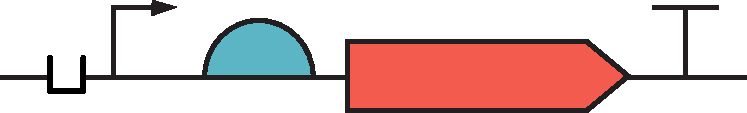
\includegraphics[scale=0.4]{figures/examples/2e-promoter2.pdf}}
	\caption{Examples where glyphs SHOULD overlap, but might not if it is more clear, e.g., with an operator site located within the 5' portion of a promoter}
	\label{exa:2e}
	\end{figure}

\item A nucleic acid \sbol{Component} SHOULD be represented using a glyph defined in \ref{apdx:symbols}.  In this case, the glyph's definition MUST be equal to or a parent of at least one of the \sbol{roles} for the \sbol{Component} or its associated \sbol{ComponentDefinition}, and SHOULD be the RECOMMENDED variant of the most specific applicable glyph.  Note that novel glyphs not defined in \ref{apdx:symbols} MAY be used, but SHOULD be proposed for adoption as described in \ref{sec:extension}.
	Examples are provided in~\ref{exa:2f}.
\actionitem{update 9c to use Unspecified}
	\begin{figure}[h!]
	\centering
	\subfigure[SHOULD]{\includegraphics[scale=0.5]{figures/examples/2f-recommended.pdf}}
	\subfigure[MAY]{\includegraphics[scale=0.5]{figures/examples/2f-custom.pdf}}
	\subfigure[SHOULD NOT]{\includegraphics[scale=0.5]{figures/examples/2f-generic.pdf}}
	\subfigure[MUST NOT]{\includegraphics[scale=0.5]{figures/examples/2f-conflict.pdf}}
	\caption{Examples of recommended, allowed, and forbidden representation of a \sbol{ComponentDefinition} comprising a sequence of promoter, 5'UTR, CDS, and terminator: (b) is allowed because it uses a custom non-conflicting symbol to encode more specific information about the particular CDS, (c) is recommended against because it uses less specific glyphs and (d) is forbidden because it use a promoter symbol to represent the terminator.}
	\label{exa:2f}
	\end{figure}
\end{enumerate}
	
	
\subsection{Labels}
The \sbol{name} of any object in a diagram is RECOMMENDED to be displayed as text within, adjacent to, or otherwise clearly visually connected to the object's associated glyph.  If no \sbol{name} is supplied, then the \sbol{displayId} MAY be used instead.
Examples are provided in~\ref{exa:5}.

	\begin{figure}[h!]
	\centering
	\includegraphics[width=3in]{figures/examples/5-labels.pdf}
	\caption{Examples of labels on glyphs.}
	\label{exa:5}
	\end{figure}


\subsection{Annotations}
Other text or graphics may be included as annotations with no constraint on their syntax or semantics.

\begin{enumerate}
\item Annotations SHOULD NOT be displayed in a way that allows them to be confused with other SBOL visual elements.
\item Annotations SHOULD NOT be used to display information that can be displayed using other SBOL visual elements.
\end{enumerate}

\subsection{Criteria for Compliance with SBOL Visual}

A diagram of a biological system is compliant with SBOL Visual if it complies with all MUST and MUST NOT requirements as specified above.
A diagram is compliant with SBOL Visual best practices if it also complies with all RECOMMENDED, SHOULD, and SHOULD NOT statements as specified above.

Importantly, note that a non-SBOL glyph can be used in a compliant
diagram when its definition is a subset or superset of definition that
does have an SBOL Visual glyph.  For example, a diagram that creates a
new glyph for a special type of promoter can be SBOL Visual compliant
even though there is an SBOL Visual glyph for a general promoter.

A piece of software or other system for producing diagrams is
compliant with SBOL Visual under the following conditions:
\begin{enumerate}
\item The system MUST be capable of producing diagrams that are
  compliant with SBOL Visual.
\item If the system can also produce diagrams that are {\em not}
  compliant with SBOL Visual, it MUST clearly distinguish to the user
  between compliant and non-compliant usage and diagrams.
\end{enumerate}



\appendix
\appendixlabels

% -----------------------------------------------------------------------------
\section{SBOL Visual Glyphs}\label{apdx:symbols}
% -----------------------------------------------------------------------------

The following pages present all current glyphs for SBOL Visual, organized by glyph families.
Each entry lists:
\begin{itemize}
\item Glyph family name
\item Associated ontology terms
\item Recommended and alternate glyphs
\item At least one example of when this glyph would be used
\item Any additional notes
\end{itemize}

\subsection{Sequence Feature Glyphs}\label{apdx:sym:feature}

These glyphs represent features of nucleic acid sequences, and include a bounding box (grey dashed box) and a recommended alignment to the nucleic acid backbone (grey dashed horizontal line).

% -----------------------------------------------------------------------------
\section{SBOL Glyphs}\label{sec:glyphs}
% -----------------------------------------------------------------------------

A glyph is a visual symbol used to represent an element in an SBOL Visual diagram.
All of the currently defined glyphs are collected in \ref{apdx:symbols}.
%
This section explains how glyphs are specified and how to add new glyphs.

Each SBOL glyph is defined by association with ontology terms, and can be used to represent any nucleic acid sequence feature that is well-described by that term.  
For SBOL 2 data models, this is formally defined as any \sbol{Component} with a compatible term within its \sbol{roles},
 i.e. one that is equal to or a child of at least one term associated with the glyph.
 
More than one glyph may share the same definition: in this case, these glyphs form a family of variants, of which precisely one MUST be designated as the RECOMMENDED glyph, which is to be used unless there are strong reasons to prefer an alternative variant.

It will also frequently be the case that a sequence feature could be represented by more than one glyph (e.g., a glyph for a specific term and a glyph for a more general term).
In such cases, it is RECOMMENDED that the most specific applicable glyph be used.

For example, a CDS may be represented as either using the CDS glyph (Sequence Ontology term SO:0000316) or the Unspecified glyph (Sequence Ontology term SO:0000001).  
Since SO:0000316 is contained by SO:0000001, the preferred glyph is CDS, rather than Unspecified.
Likewise, a CDS may be represented by either a pentagonal glyph or an arrow glyph, but the pentagon is the RECOMMENDED variant, and so it is likewise preferred.  

\actionitem{Make a figure for this example}

\subsection{Requirements for Glyphs}

A number of requirements are placed on SBOL Visual glyphs in order to
ensure both the clarity of diagrams and the ease with which they can
be constructed:
\begin{enumerate}
\item A glyph SHOULD have its meaning defined by associating the glyph with at least one ontology definition.
	Definitions are RECOMMENDED to be from the Sequence Ontology for nucleic acid components and from Systems Biology Ontology for other components and interactions.  
	If no applicable terms are available in the preferred ontology, proposal of a new glyph SHOULD be accompanied by a request to the ontology maintainers to add a term for the undefined entity.  
\item A glyph MUST be relatively easy to sketch by hand (e.g., no high-complexity images or precise angles required).
\item A glyph specification MUST include a rectangular bounding box indicating its extent in space.
\item A glyph specification MUST include a horizontal rule for its RECOMMENDED vertical alignment with the \sbol{ComponentDefinition} backbone.
\item A glyph specification MUST indicate which portions of the glyph are the ``interior'' for purposes of color fill.
\item A glyph specification SHOULD show the glyph in its preferred relative scale with respect to other glyphs.
\item A glyph SHOULD be specified using only solid black lines (leaving color and style to be determined by the user, as noted below).
\item A glyph SHOULD NOT be similar enough to be easily confused with any other glyph when written by hand, or when scaled either vertically, horizontally, or both.
\item A glyph SHOULD be asymmetric on the horizontal axis. Vertical asymmetry is also preferred when possible.
\item If a glyph can represent components of highly variable size or structural complexity, the glyph SHOULD be able to be scaled horizontally to indicate relative property value.
\item A glyphs SHOULD NOT include text.
\end{enumerate}

\actionitem{example of a glyph specification: promoter}

\subsection{Reserved Visual Properties}

SBOL Visual aims to allow as much flexibility and freedom as possible in how diagrams are organized, presented, and styled.
%
To this end, a number of aspects of presentation are generally reserved for the communication of other types of information by the creator of a diagram.
%
When using a glyph in a diagram, the following choices in glyph presentation are thus explicitly intended to be alterable:
\begin{enumerate}
\item The lines of a glyph MAY be given any line thickness and style
\item The interior of a glyph MAY be given any fill color.
\item The scale of glyphs are RECOMMENDED to be kept consistent with their specification and throughout a diagram, but can be altered if desired, particularly to convey additional information (e.g., length of a sequence).
\item Minor styling effects MAY be chosen (e.g., shadow, corner styling, other "font-level" customization)
\end{enumerate}
Exceptions may be made for certain glyphs in special cases, but such cases are expected to be rare and strongly motivated.

\actionitem{examples of stylistic variation}


\subsection{Extending the Set of Glyphs}\label{sec:extension}
The collection of SBOL Visual glyphs is not expected to provide
complete coverage of all of the types of component that people will
wish to include in genetic diagrams, particularly given the ongoing
evolution of synthetic biology as an engineering discipline.
%
As the need for new diagram elements or new practices of usage emerge,
new glyphs or glyph definitions are expected to be added to SBOL
Visual.
%
In particular, the following three classes of changes are expected to occur regularly,
and the SBOL development community will maintain clear processes for
proposal and adoption of changes of this type:
\begin{itemize}
\item New glyphs, either representing a type of component that
  previously lacked a glyph or enabling a distinction between types of
  component previously represented by the same glyph.
\item Additional glyph variants, accompanied by compelling use cases
  that cannot be adequately addressed by the existing glyph variants.
\item Additional definitions for a glyph, capturing an alternate
  meaning that is useful to humans but existing within a disjoint
  branch of the Sequence Ontology.
\end{itemize}

In order to support the coherent extension of SBOL Visual, 
whenever a diagram creator uses a glyph not found in \ref{apdx:symbols}, 
the creator SHOULD submit it to be considered for inclusion in an updated version of the standard following the processes for adding new glyphs found on the community website at \url{http://sbolstandard.org}






\subsection{Molecular Species Glyphs}\label{apdx:sym:species}

These glyphs represent molecular species in a diagram, and include a bounding box (grey dashed box) but are not connected to any nucleic acid backbone.

% Autogenerated glyph page collection, do not edit by hand
\twotwozeronopage{
\includepdf[pagecommand={},pages={1-}]{glyphscript/Glyphs/FunctionalComponents/complex.pdf}

\includepdf[pagecommand={},pages={1-}]{glyphscript/Glyphs/FunctionalComponents/dsNA.pdf}

\includepdf[pagecommand={},pages={1-}]{glyphscript/Glyphs/FunctionalComponents/macromolecule.pdf}

\includepdf[pagecommand={},pages={1-}]{glyphscript/Glyphs/FunctionalComponents/no-glyph-assigned.pdf}

\includepdf[pagecommand={},pages={1-}]{glyphscript/Glyphs/FunctionalComponents/protein.pdf}
\includepdf[pagecommand={},pages={1-}]{glyphscript/Glyphs/FunctionalComponents/simple-chemical.pdf}

\includepdf[pagecommand={},pages={1-}]{glyphscript/Glyphs/FunctionalComponents/ssNA.pdf}
\includepdf[pagecommand={},pages={1-}]{glyphscript/Glyphs/FunctionalComponents/unspecified.pdf}
}


\subsection{Interaction Glyphs}\label{apdx:sym:interaction}

These glyphs are different forms of ``arrow'' representing interactions between sequence features and/or molecular species. As arrows, they are extensible and do not have a separately identified bounding box.

% Autogenerated glyph page collection, do not edit by hand
\twotwozeronopage{
\includepdf[pagecommand={},pages={1-}]{glyphscript/Glyphs/Interactions/control.pdf}
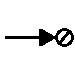
\includepdf[pagecommand={},pages={1-}]{glyphscript/Glyphs/Interactions/degradation.pdf}
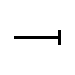
\includepdf[pagecommand={},pages={1-}]{glyphscript/Glyphs/Interactions/inhibition.pdf}
\includepdf[pagecommand={},pages={1-}]{glyphscript/Glyphs/Interactions/process.pdf}
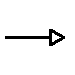
\includepdf[pagecommand={},pages={1-}]{glyphscript/Glyphs/Interactions/stimulation.pdf}
}


\twoonezero{
\subsection{Interaction Node Glyphs}\label{apdx:sym:interactionnodes}

These glyphs are placed at the junctions of edges to represent biochemical processes, and include a bounding box (grey dashed box) but are not connected to any nucleic acid backbone. Grey dashed lines provide examples of how edges may connect to the glyph.
}

% Autogenerated glyph page collection, do not edit by hand
\twoonezeronopage{

\includepdf[pagecommand={},pages={1-}]{glyphscript/Glyphs/InteractionNodes/association.pdf}
\includepdf[pagecommand={},pages={1-}]{glyphscript/Glyphs/InteractionNodes/dissociation.pdf}
\includepdf[pagecommand={},pages={1-}]{glyphscript/Glyphs/InteractionNodes/process.pdf}
}


% -----------------------------------------------------------------------------
\section{Examples}\label{sec:examples}
% -----------------------------------------------------------------------------

This section contains prototypical examples, including use of all
current glyphs to attempt to ensure that their use is clear.

\begin{figure}[h!]
\includegraphics[scale=0.5]{figures/apdx-examples/apdx-exa1.pdf}
\caption{DNA sequence for a functional unit in which the pTet promoter and an anonymous ribosome entry site regulate expression of a coding sequence for GFP, ended by a terminator.}
\label{f:apdx:exa1}
\end{figure}

\begin{figure}[h!]
\includegraphics[scale=0.5]{figures/apdx-examples/apdx-exa2.pdf}
\caption{The same functional unit as in \ref{f:apdx:exa1}, with additional assembly-focused information: there is a 5' overhang before the promoter, a 3' overhand after the terminator, and an assembly scar between the promoter and the ribosome entry site left over from a prior step of assembly.}
\label{f:apdx:exa2}
\end{figure}

\begin{figure}[h!]
\includegraphics[scale=0.5]{figures/apdx-examples/apdx-exa3.pdf}
\caption{Promoter pTet stored in a circular plasmid. The promoter is prepared for being cut out of the plasmid: it is preceded by a 5' sticky end restriction site and followed by a 3' stick end restriction site.  In addition, the plasmid has been bar-coded with a signature and has its origin of replication marked.}
\label{f:apdx:exa3}
\end{figure}

\begin{figure}[h!]
\includegraphics[scale=0.5]{figures/apdx-examples/apdx-exa4.pdf}
\caption{Promoter stored in a plasmid as in \ref{f:apdx:exa3}, except that the restriction sites before and after the promoter are blunt-end.}
\label{f:apdx:exa4}
\end{figure}

\begin{figure}[h!]
\includegraphics[scale=0.5]{figures/apdx-examples/apdx-exa5.pdf}
\caption{Promoter stored in a plasmid as in \ref{f:apdx:exa3}, except that the cut structure of the restriction sites before and after the promoter is not specified.}
\label{f:apdx:exa5}
\end{figure}

\begin{figure}[h!]
\includegraphics[scale=0.5]{figures/apdx-examples/apdx-exa6.pdf}
\caption{Promoter stored in a plasmid as in \ref{f:apdx:exa3}, except that there is a ribonuclease sites after the promoter rather than restriction sites flanking it.}
\label{f:apdx:exa6}
\end{figure}

\begin{figure}[h!]
\includegraphics[scale=0.5]{figures/apdx-examples/apdx-exa7.pdf}
\caption{Detailed design of a promoter, in which the transcription start site is preceded by two operator sites where regulators bind, and the whole is flanked by insulators.}
\label{f:apdx:exa7}
\end{figure}

\begin{figure}[h!]
\includegraphics[scale=0.5]{figures/apdx-examples/apdx-exa8.pdf}
\caption{Promoter regulating the production of an engineered composite sequence that includes RNA and protein stability elements at its 3' end, as well as an internal site for protease cleavage, as well as the expansion of the composite to show it contains a ribosome entry site. coding sequence, and other omitted details.  Single residue locations of interest are indicated for the DNA (before the promoter), RNA (after the ribosome entry site), and protein (in the CDS).}
\label{f:apdx:exa8}
\end{figure}

\begin{figure}[h!]
\includegraphics[scale=0.5]{figures/apdx-examples/apdx-exa9.pdf}
\caption{DNA sequence with three primer binding sites.}
\label{f:apdx:exa9}
\end{figure}

\begin{figure}[h!]
\includegraphics[scale=0.5]{figures/apdx-examples/apdx-exa10.pdf}
\caption{The same functional unit as in \ref{f:apdx:exa1}, except that information about the CDS is missing, leaving it to fall back on the default unspecified glyph.}
\label{f:apdx:exa10}
\end{figure}

\begin{figure}[h!]
\includegraphics[scale=0.5]{figures/apdx-examples/apdx-exa11.pdf}
\caption{Promoter regulating the expression of GFP, which is also regulated by an aptamer between it and the poly-A tail of the transcript. The promoter can be cut out by a pair of recombinase target sites, which are acted on by the Flp protein.  The whole construct is stored in a circular plasmid with an origin of replication and also an origin of transfer.}
\label{f:apdx:exa11}
\end{figure}

\begin{figure}[h!]
\includegraphics[scale=0.5]{figures/apdx-examples/apdx-exa12.pdf}
\caption{Promoter stimulated by the CDS that it regulates.}
\label{f:apdx:exa12}
\end{figure}

\begin{figure}[h!]
\includegraphics[scale=0.5]{figures/apdx-examples/apdx-exa13.pdf}
\caption{Constitutive production of TetR, except that information about the protein is missing, leaving it as the default unspecified glyph. TetR represses the pTet promoter, which is regulating production of GFP.  The diagram of GFP production explicitly includes the intermediate mRNA and the degradation of both the mRNA and protein products.}
\label{f:apdx:exa13}
\end{figure}

% Figure black magic: adjust the size here as needed to get the spacing on the last page of the section correct.
\begin{figure}[h!]
\vspace{2in}
\end{figure}


% -----------------------------------------------------------------------------
\section{Relationship to SBOL Visual 1.0}\label{sec:sbol1}
% -----------------------------------------------------------------------------

SBOL Visual 1.1 differs from SBOL Visual 1.0 in the following major ways:
\begin{itemize}
\item The relationship between diagrams and the SBOL data model is made explicit.
\item A number of requirements and best practices are specified for glyphs and diagrams, including:
	\begin{itemize}
	\item Glyphs include information on interior, bounding box, and recommended backbone alignment.
	\item Glyphs are required to have their bounding boxes contact the nucleic acid backbone.
	\item Nucleic acid diagrams now require the nucleic acid backbone line, and the number of lines allowed in various circumstances is constrained.
	% glyph overlaps needs to be handled be SEP
	%\item Glyphs are not allowed to overlap in bounding-box unless 
	\item Explicit statement of when a glyph can and cannot be used to represent a particular element of a diagram.
	\end{itemize}
\item Labels that name objects are distinguished from other types of textual annotation.
\item Explicit statement of which aspects of a symbol are {\em not} controlled.
\item Symbol variants are now supported.
\end{itemize}

In addition, the collection of glyphs have been expanded and modified in the following ways:
\todo[inline]{work this through in detail per the various SEPs}

%
%\begin{itemize}
%\item Ribonuclease Site has been assigned SO:0001977.
%\item 5' Sticky End Restriction Site has been assigned SO:0001975.
%\item 3' Sticky End Restriction Site has been assigned SO:0001976.
%\item Signature has been assigned SO:0001978.
%\end{itemize}
%
%% I have verified that there are all as desired.
%In addition, the following changes have been made to ontology links:
%\begin{itemize}
%\item The symbol for 5'UTR (SO:0000204) has been generalized from its former definition as Ribosome Entry Site (SO:0000139).
%\item User-defined component has been assigned a definition as Sequence Feature (SO:0000110).
%\item RNA stability element's can be defined as either SO:0001957 or SO:0001546.
%\item Restriction site can be defined as either SO:0001687 or SO:0000061.
%\item 5' Overhang Site and 3' Overhang Site were erroneously listed with their ontology terms exchanged; this has been fixed.
%\end{itemize}
%


\newpage
\label{s:bibliography}
\bibliography{sbol}

\end{document}
